\documentclass[a4paper,10pt,twoside]{article}
\title
{
\LARGE BITS F464 Machine Learning \\
\LARGE Multi-Layer Perceptron
}
\usepackage[left=2cm, right=2cm, top=1.5cm]{geometry}
\usepackage{xcolor}
\usepackage{ragged2e}
\usepackage{comment}
\usepackage{graphicx}
\usepackage{subfig}
\usepackage{amsmath, amsfonts}
\usepackage[english]{babel}
\date{}
\author{}
\begin{document}
\maketitle
%===================================================================================================================%
\section*{\textcolor{blue}{1. Introduction:}}
In this report, we try to analyse the performance (accuracy, fscore, recall and precision) of a neural network that we built using NumPy. The implementation of this network is similar to that of Keras and the whole code has been written in a completely modularized fashion.

\section*{\textcolor{blue}{2. Data Preprocessing:}}
The dataset $housepricesdata.csv$ contained 1460 data points, each containing 10 input features (representing house features) and one binary target variable (representing if the house price is above or below the median price). In the preprocessing stage, all features were standardized and randomly split into \textit{train\_set} and \textit{test\_set} (80-20 split ratio).

\section*{\textcolor{blue}{3. Activation functions:}}
\begin{itemize}
\item{linear: $y = x$}
\item{tanh: $y$ = $\frac{e^x - e^{-x}}{e^x + e^{-x}}$}
\item{sigmoid: $y$ = $\frac{1}{1 + e^{-x}}$}
\item{ReLU: $y$ = $max(0, x)$}
\end{itemize}

\section*{\textcolor{blue}{4. Loss function:}}
\begin{itemize}
\item{$L_n = -t_nlog(y_n)-(1-t_n)log(1-y_n)$} 
\end{itemize}

\section*{\textcolor{blue}{5. Network Architecture:}}
\subsection*{\textcolor{red}{5.1 Two-Layer NN}}
The first model we built was a 2-layer neural network (i.e. with one hidden layer). We experimented with activations like linear, ReLU and tanh for the hidden layer. The input layer had 10 neuron units with a ReLU activation (for best results. A slight drop in accuracy was observed when linear activation was used for the input layer). The final layer had an activation of sigmoid for binary classification. Output value greater than or equal to 0.5 was taken to represent positive classes and less than 0.5 to represent negative classes.
\texttt{np.random.random()} and \texttt{np.random.randn()} methods were used to randomly initialize weights and biases associated network to initialize the weights according to a Uniform or Guassian distribution respectively. Best results were obtained using uniformly distributed weights/biases with a seed=5 and 4 hidden neurons with ReLU and learning\_rate=0.001 with 20000 training epochs. The loss was observed to have more fluctuations using this configuration after 40000 epochs and thus lowering the accuracy. The avg. loss using this configuration was observed to be 0.7 (per data point). The highest accuracy achieved by this model using this configuration was 87.67\% and the lowest accuracy was 80\% with an average accuracy of 84\%.

\subsection*{\textcolor{red}{5.2 Three-Layer NN}}
The second model we built and experimented with was a three layer neural network. The accuracy of the three layer neural network was found to be better than that of the two layer network. Both the hidden layers had 5 neurons with ReLU activation for optimal results. Training the network, in this case, required more iterations as there were more number of parameter to be tuned than the two layer network. The optimal number of neurons for both hidden layers were chosen accordingly as suggested in research article \textit{Review on Methods to Fix Number of Hidden Neurons in Neural Networks} by Gnana Sheela et al. Once again, best results were obtained using uniform distribution of weights with learning\_rate=0.01 and 40000 iterations. The following combination yielded the highest accuracy of 91.43\% with a minimum accuracy of 80\% and an average accuracy of 86\%.

\section*{\textcolor{blue}{6. Conclusion:}}
\begin{itemize}
\item{In general, a three layer network performs better than a two layer network. Adding more layers/more neurons to the hidden layers provides more trainable parameters which help the network to fit the model in a better way. But the drawback of adding multiple layers/mulitple neurons is that, the model requires more iterations to train. In this case, there is a higher chance that the model might overfit the data, and hence giving a low testing accuracy.}
\item{A lower learning rate requires more iterations to converge, but conversely, using a higher learning rate might lead to fluctuation in the loss/exploding gradient.}
\item{Different initialization of weights leads to convergence of the model at different local minima (initializations mentioned above).}
\item{Different activation functions for the hidden layers provides drastically varying results. We	 have used ReLU (Rectified Linear) which is by and the far, the de-facto standard activation used for hidden layers. Other activations like tanh or sigmoid gave very low accuracy as compared to that of ReLU. ReLU suffers from the \emph{dying neuron problem}, in which the output of a neuron might be 0 for most of the training (i.e. that neuron is not contributing to the network), and hence we tried using leaky-ReLU, but the accuracy was found to more or less the same.}
\end{itemize}
[results on next page]

\section*{\textcolor{blue}{7. Additional Work:}}
\begin{itemize}
\item{\textcolor{red}{SGD Momentum and Decay}
\newline				
$M_t = \beta M_{t-1} + (1 - \beta)\nabla E$
\newline
$W = W - \eta M_t$
}
\item{\textcolor{red}{RMSprop}
\newline
$V_t = \beta V_{t-1} + (1 - \beta)(\nabla E)^2$
\newline
$W = W - \eta \frac{\nabla E}{\sqrt{V_t} + \epsilon}$
}
\item{\textcolor{red}{Adam}
\newline
$M_t = \beta M_{t-1} + (1 - \beta_1)\nabla E$
\newline
$V_t = \beta V_{t-1} + (1 - \beta_2)(\nabla E)^2$
\newline
$\hat{M_t} = \frac{M_t}{1 - \beta_1^t}$; $\hat{V_t} = \frac{V_t}{1 - \beta_2^t}$
\newline
$W = W - \eta \frac{\hat{M_t}}{\sqrt{\hat{V_t}} + \epsilon}$
}
\end{itemize}

\onecolumn
\section*{\textcolor{blue}{8. Results:}}
\begin{figure}[h!]
\centering
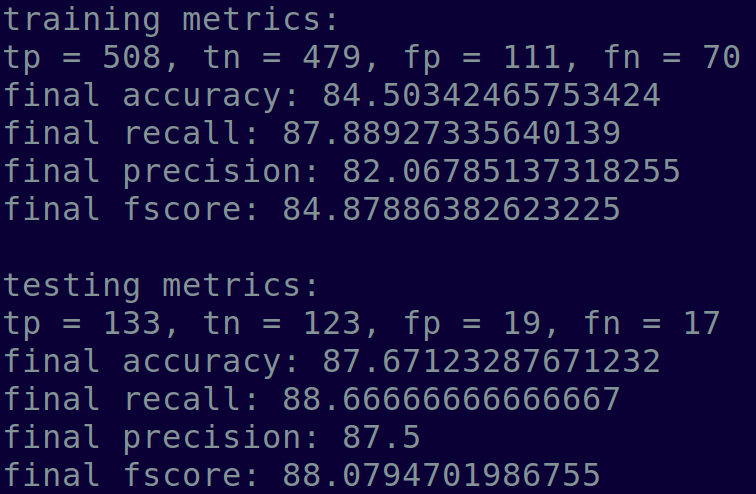
\includegraphics[scale=1.0, width=5cm]{Fig1.png}
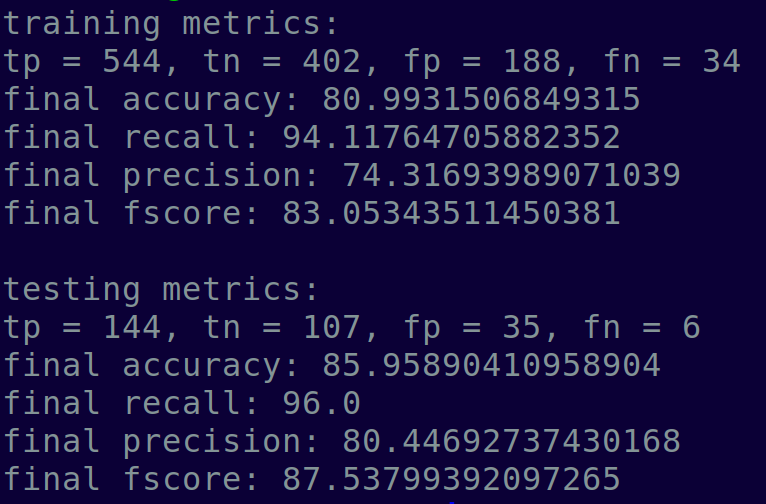
\includegraphics[scale=1.0, width=5cm]{Fig2.png}
\caption*{2-Layer NN using uniform distribution}
\end{figure}

\begin{figure}[h!]
\centering
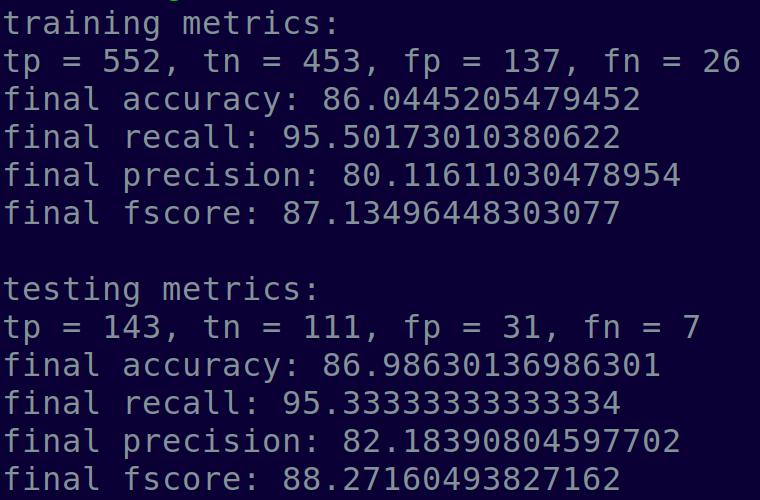
\includegraphics[scale=1.0, width=5cm]{Fig3.png}
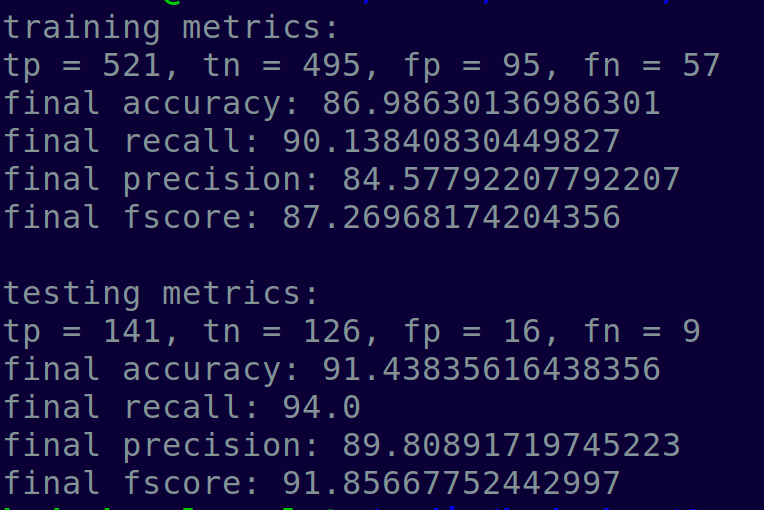
\includegraphics[scale=1.0, width=5cm]{Fig4.png}
\caption*{3-Layer NN using uniform distirbution}
\end{figure}

\begin{figure}[h!]
\centering
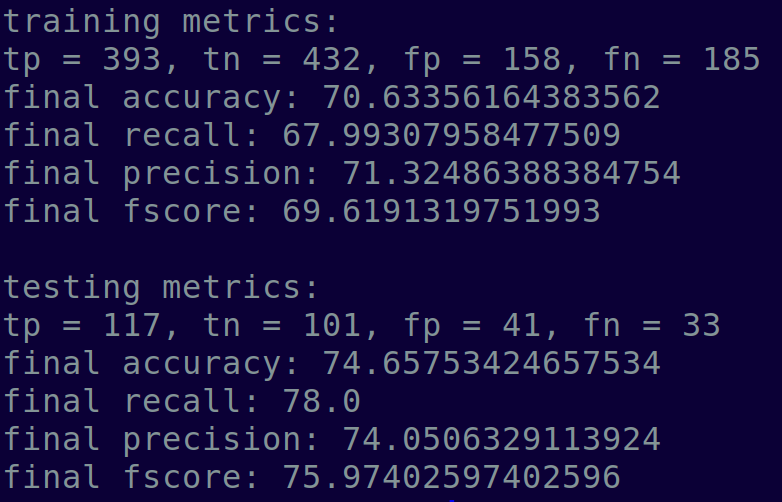
\includegraphics[scale=1.0, width=5cm]{Fig5.png}
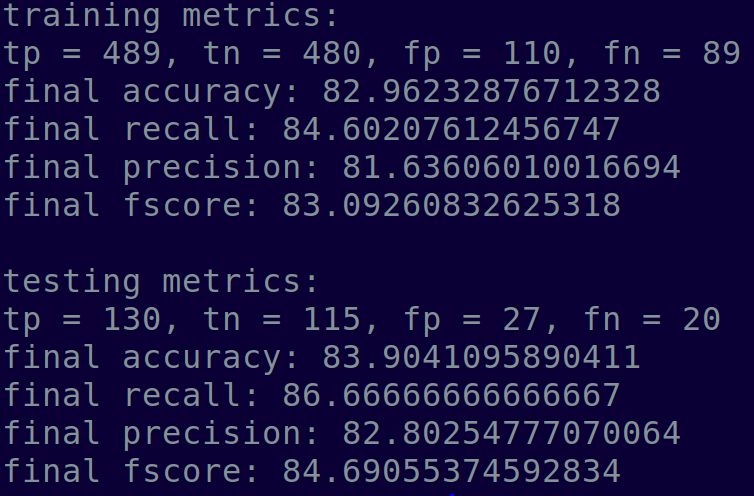
\includegraphics[scale=1.0, width=5cm]{Fig6.png}
\caption*{2-Layer NN using normal distirbution}
\end{figure}

\begin{figure}[h!]
\centering
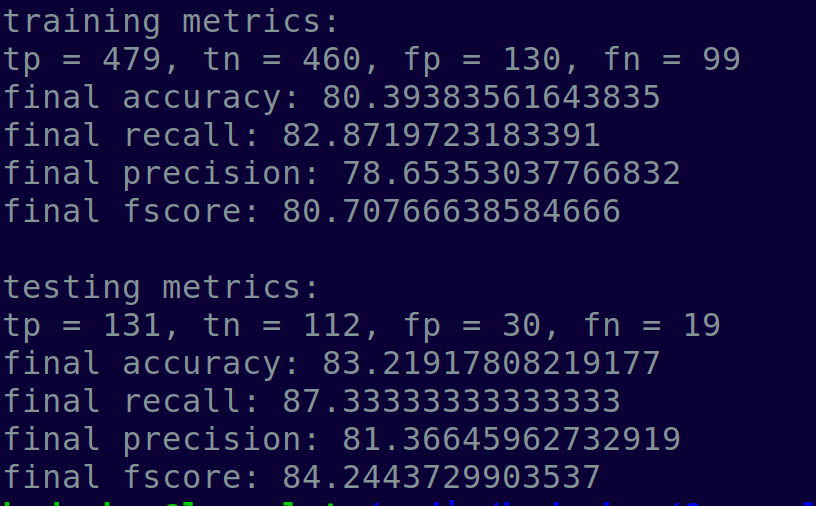
\includegraphics[scale=1.0, width=5cm]{Fig7.png}
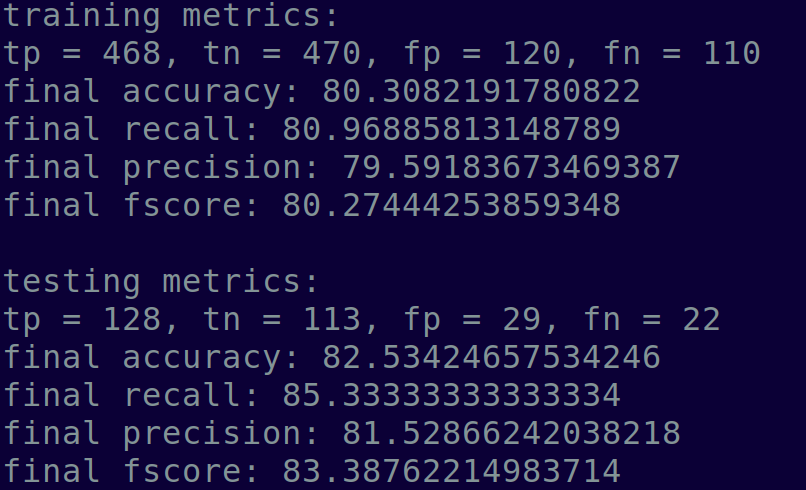
\includegraphics[scale=1.0, width=5cm]{Fig8.png}
\caption*{3-Layer NN using normal distirbution}
\end{figure}

\begin{figure}[h!]
\centering
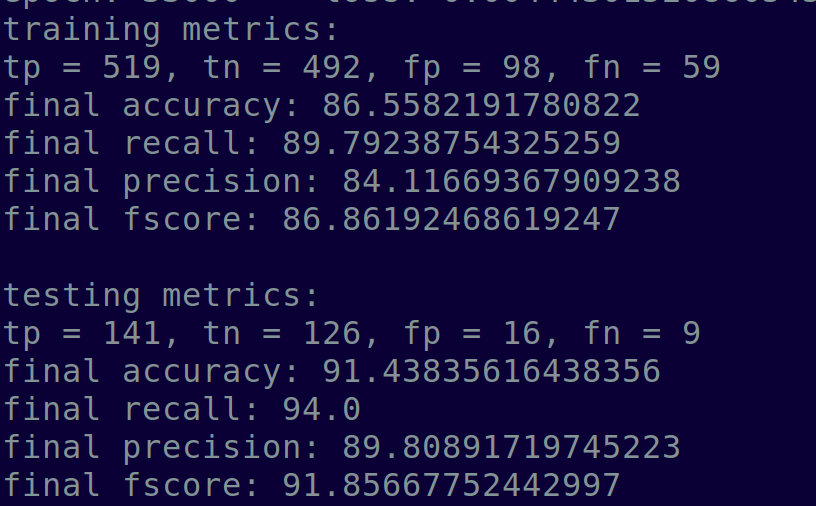
\includegraphics[scale=1.0, width=5cm]{Fig9.png}
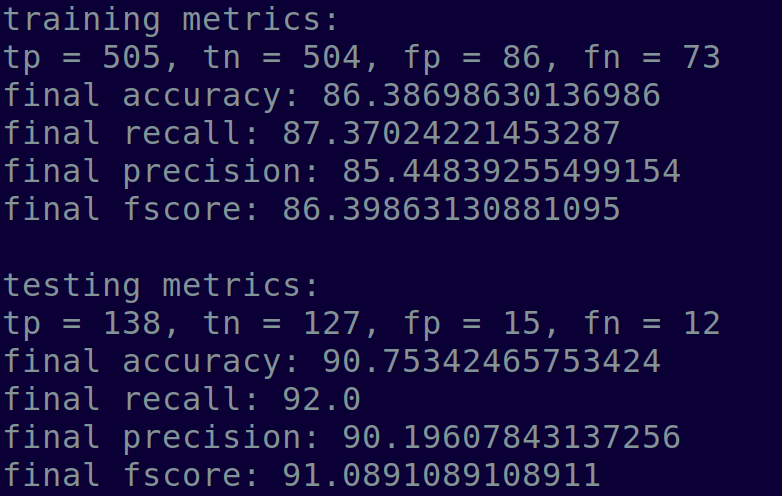
\includegraphics[scale=1.0, width=5cm]{Fig10.png}
\caption*{3-Layer NN using uniform distirbution with momentum and decay}
\end{figure}


\newpage
\onecolumn
\section*{\textcolor{blue}{9. Additional Results:}}
\begin{figure}[h!]
\centering
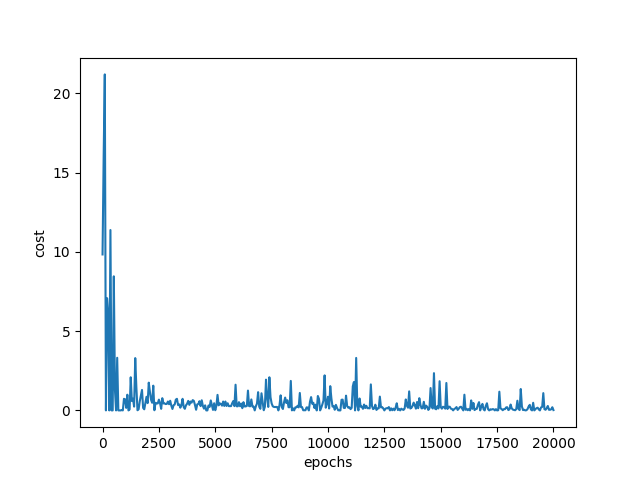
\includegraphics[scale=1.0, width=5cm]{Fig31_Adam.png}
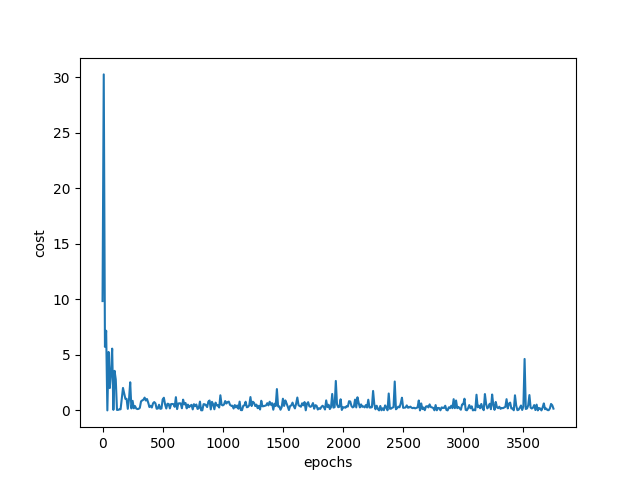
\includegraphics[scale=1.0, width=5cm]{Fig32_RMSprop.png}
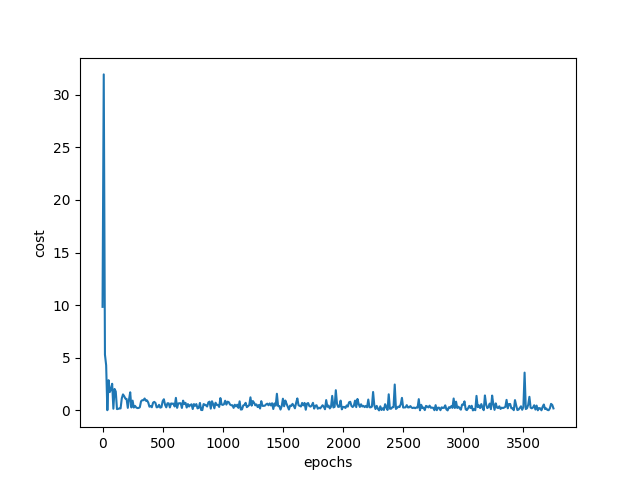
\includegraphics[scale=1.0, width=5cm]{Fig33_SGD_momentum.png}
\caption*{Loss vs Epochs for Adam, RMSprop and Momentum respectively}
\end{figure}

\begin{figure}[h!]
\centering
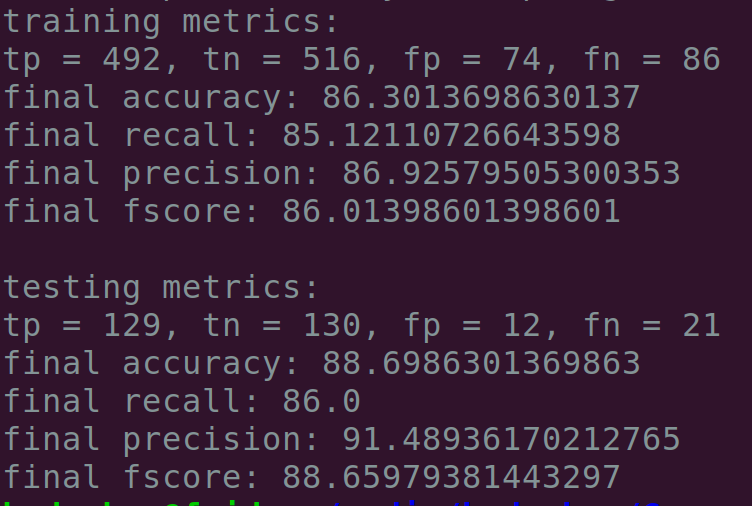
\includegraphics[scale=1.0, width=5cm]{Fig41_Adam.png}
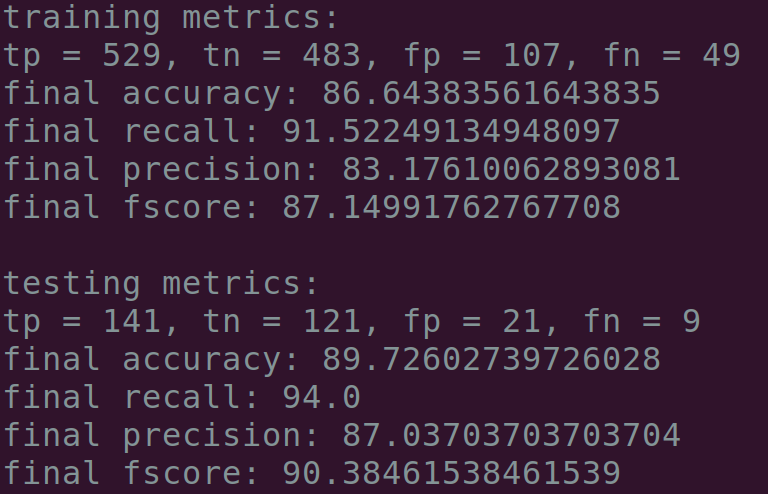
\includegraphics[scale=1.0, width=5cm]{Fig42_RMSprop.png}
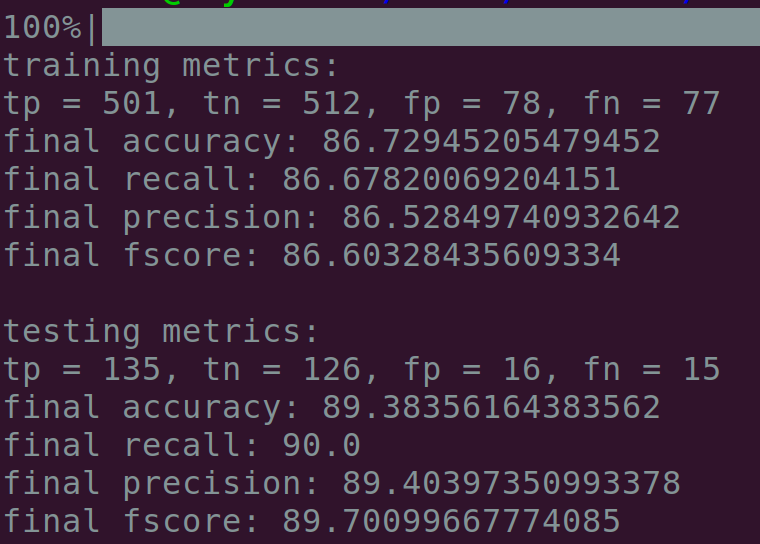
\includegraphics[scale=1.0, width=5cm]{Fig43_SGD_momentum.png}
\caption*{3-Layer NN with Adam, RMSprop and Momentum respectively for 3750 epochs}
\end{figure}
%=================================================================================================================%
\end{document}
